\documentclass[10pt,english,aspectratio=169]{beamer}
% Use notes or hide notes or show only notes or handout


\usetheme{default}

\usepackage{xstring}
\usepackage{pgfpages}
%\makeatletter
%\IfSubStr{\@classoptionslist}{handout}
%  {\pgfpagesuselayout{2 on 1}[letterpaper,border shrink=5mm]}
%  {}
%\makeatother

\usepackage{amsmath,amssymb,amsthm}
\usepackage{stmaryrd}
\usepackage{enumerate}
\usepackage{stfloats}
\usepackage{bbm}
\usepackage{pdfpages}
\usepackage{framed}
\usepackage{tabularx}
\usepackage{scalerel}

\usepackage[most]{tcolorbox}
\tcbset{highlight math style={enhanced,
  colframe=white,colback=yellow!15,arc=8pt,boxrule=1pt,
  }}
  
\usepackage{tikz,pgf,pgfplots}
\usepackage{tikz-3dplot}
\usepackage{algorithm,algorithmic}
\usepgflibrary{shapes}
\usetikzlibrary{%
  arrows,%
  arrows.meta,
  backgrounds,
  shapes.misc,% wg. rounded rectangle
  shapes.arrows,%
  shapes,%
  calc,%
  chains,%
  matrix,%
  positioning,% wg. " of "
  scopes,%
  decorations.pathmorphing,% /pgf/decoration/random steps | erste Graphik
  shadows,%
  backgrounds,%
  fit,%
  petri,%
  quotes
}

\tikzset{background rectangle/.style={
    fill=white,
  },
  use background/.style={    
    show background rectangle
  }
}

\setbeamersize{text margin left=10mm,text margin right=35mm}

\pgfplotsset{compat=1.12}

%\usetheme{Frankfurt}
%\usecolortheme{ldpc}
\useinnertheme{rounded}
\usecolortheme{whale}
\usecolortheme{orchid}

\newcommand{\ul}[1]{\underline{#1}}
\renewcommand{\Pr}{\mathbb{P}}

%% Setup slides and notes
\makeatletter
\IfSubStr{\@classoptionslist}{notes} { \IfSubStr{\@classoptionslist}{hide} {}{\IfSubStr{\@classoptionslist}{only} {}{\setbeameroption{show notes on second screen=right}}} }{}
\makeatother
%\setbeamertemplate{note page}{\pagecolor{yellow!5}\vfill\insertnote\vfill}

\newcommand{\getpdfpages}[2]{\begingroup
  \setbeamercolor{background canvas}{bg=}
  \addtocounter{framenumber}{1}
  \includepdf[pages={#1},%
  pagecommand={%
    \expandafter\def\expandafter\insertshorttitle\expandafter{%
      \insertshorttitle\hfill\insertframenumber\,/\,\inserttotalframenumber}}%
  ]{#2}
  \endgroup}

\newcommand{\backupbegin}{
   \newcounter{finalframe}
   \setcounter{finalframe}{\value{framenumber}}
}
\newcommand{\backupend}{
   \setcounter{framenumber}{\value{finalframe}}
}

 \setbeamercolor{bibliography entry author}{fg=black}
 \setbeamercolor{bibliography entry title}{fg=black}
 \setbeamercolor{bibliography entry location}{fg=black}
 \setbeamercolor{bibliography entry note}{fg=black}
 
 \setbeamerfont{bibliography item}{size=\footnotesize}
 \setbeamerfont{bibliography entry author}{size=\footnotesize}
 \setbeamerfont{bibliography entry title}{size=\footnotesize}
 \setbeamerfont{bibliography entry location}{size=\footnotesize}
 \setbeamerfont{bibliography entry note}{size=\footnotesize}
 \setbeamertemplate{bibliography item}{\insertbiblabel}
 
\newlength\tikzwidth
\newlength\tikzheight


\newcommand{\mc}[1]{\mathcal{#1}}
\newcommand{\mbb}[1]{\mathbb{#1}}
%\newcommand{\expt}{\mbb{E}}
%\newcommand{\dd}{\mathrm{d}}
\newcommand{\Interior}[1]{\ensuremath{{#1}^{\circ}}}
\newcommand{\Closure}[1]{\ensuremath{\overline{#1}}}
\newcommand{\Complement}[1]{\ensuremath{{#1}^{c}}}

\newcommand{\Expect}{\ensuremath{\mathrm{E}}}
\newcommand{\vecnot}{\underline}
\newcommand{\RealNumbers}{\ensuremath{\mathbb{R}}}
\newcommand{\RationalNumbers}{\mathbb{Q}}
\newcommand{\ComplexNumbers}{\mathbb{C}}
\newcommand{\Real}{\mathrm{Re}}
\newcommand{\Span}{\mathrm{span}}
\newcommand{\Rank}{\mathrm{rank}}
\newcommand{\Nullity}{\mathrm{nullity}}
\newcommand{\Trace}{\mathrm{tr}}
\newcommand{\Diag}{\mathrm{diag}}
\newcommand{\dd}{\mathrm{d}}
\DeclareMathOperator*{\esssup}{ess\,sup}

% Use < , > inner product
\newcommand{\inner}[2]{{\left\langle #1 \mskip2mu , #2 \right\rangle}}
\newcommand{\tinner}[2]{{\langle #1 \mskip1mu , #2 \rangle}}

% Use < | > inner product
%\newcommand{\inner}[2]{{\left\langle #1 \mskip2mu \middle| \mskip2mu #2 \right\rangle}}
%\newcommand{\tinner}[2]{{\langle #1 \mskip1mu | \mskip1mu  #2 \rangle}}




\def\checkmark{\tikz\fill[scale=0.4](0,.35) -- (.25,0) -- (1,.7) -- (.25,.15) -- cycle;}
\def\greencheck{{\color{green}\checkmark}}
\def\scalecheck{\resizebox{\widthof{\checkmark}*\ratio{\widthof{x}}{\widthof{\normalsize x}}}{!}{\checkmark}}
\def\xmark{\tikz [x=1.4ex,y=1.4ex,line width=.2ex, red] \draw (0,0) -- (1,1) (0,1) -- (1,0);}
\def\redx{{\color{red}\xmark}}

\renewcommand{\footnotesep}{-2pt}

\usetikzlibrary{3d}\makeatletter \tikzoption{canvas is xy plane at z}[]{%
   \def\tikz@plane@origin{\pgfpointxyz{0}{0}{#1}}%
   \def\tikz@plane@x{\pgfpointxyz{1}{0}{#1}}%
   \def\tikz@plane@y{\pgfpointxyz{0}{1}{#1}}%
   \tikz@canvas@is@plane } \makeatother

\begin{document}

\title{ECE 586: Vector Space Methods \\ Lecture 22: Alternating Projection}
\author{Henry D. Pfister \\ Duke University}
\date{}
%\date{August 20th, 2020}
%\maketitle

\setbeamertemplate{navigation symbols}{}

\begin{frame}[plain]
	\titlepage
	
	\note{
		\vspace{8mm}
		\begin{enumerate}
			\setlength\itemsep{3mm}
			\color{red}
			\item Welcome to the 11th video lecture for ECE 586, Vector Space Methods. \\[2mm]
			Today, we'll finish our discussion of subspaces and bases and then move on to linear transforms.
		\end{enumerate}
	}
\end{frame}

\addtocounter{framenumber}{-1}
\setbeamertemplate{navigation symbols}{\textcolor{blue}{\footnotesize \insertframenumber ~/ \inserttotalframenumber}}









\begin{frame}{Alternating Projection for Subspaces}

Let \textcolor{blue}{$P_{U}$ and $P_{W}$ be orthogonal projections onto closed subspaces $U$ and $W$} of a Hilbert space $V$. For an arbitrary $\vecnot v_{0}\in V$, what is the behavior of the vector sequence $\vecnot{v}_n$ generated by \textcolor{blue}{alternating projection}:
\begin{equation*}
\vecnot v_{n+1}=\begin{cases}
P_{U}\vecnot v_{n} & \text{if }n\text{ is even}\\
P_{W}\vecnot v_{n} & \text{if }n\text{ is odd}.
\end{cases}
\end{equation*}
Since $P_{U}\vecnot v=\vecnot v$ (resp. $P_{W}\vecnot v=\vecnot v$) if and only if $\vecnot v\in U$ (resp. $\vecnot v\in W$), it is easy to see that any vector $\vecnot v\in U\cap W$ is a fixed point of this recursion.

\vspace{3mm}

Letting $P_{U\cap W}$ denote the orthogonal projection onto $U\cap W$, one can show that the \textcolor{blue}{sequence $\vecnot v_{n}$ converges to $P_{U\cap W}\vecnot v_{0}$}.

\vspace{2mm}

\begin{theorem}
The sequence $\vecnot v_{n}$ converges to $P_{U\cap W}\vecnot v_{0}$, its projection onto $U\cap W$.
\end{theorem}

\begin{tikzpicture}[overlay,remember picture,shift={(11.8,0.5)},scale=0.6]
  \begin{axis}[font=\large,width=2.5in,height=2.5in,axis lines=middle,xmin=-3.5,xmax=3.5,ymin=-3.5,ymax=3.5,grid=both]
	\addplot[red,mark=none,domain=-3.5:3.5,very thick] {x};
	\addplot[blue,mark=none,domain=-3.5:3.5,very thick] {x/2};
	\node[label={180:{\textcolor{red}{$U$}}}] at (axis cs:2.95,2.95) {};
	\node[label={270:{\textcolor{blue}{$W$}}}] at (axis cs:2.75,1.375) {};
	\end{axis}
\end{tikzpicture}

\end{frame}

% Farkas Lemma Alternative?

\begin{frame}{4.6: Projection onto Hyperplane Subspaces}

\vspace{-5mm}

The orthogonal projection of $\vecnot v\in V$ onto a 1D subspace $W=\text{span}(\vecnot w)$ is \vspace{-0.5mm}
\[
P_{W}(\vecnot v)=\frac{\inner{ \vecnot v}{\vecnot w} }{\left\Vert \vecnot w\right\Vert ^{2}}\vecnot w.
\]
%\vspace{-0.5mm}
%\hrule
%\vspace{1.75mm}

\vspace{2mm}

\visible<2->{%
A subset of $V$ that \textcolor{blue}{satisfies a single linear equality} of the form $\inner{ \vecnot v}{\vecnot w} =0$
is a subspace $U \subset V$ with \textcolor{blue}{co-dimension one} (i.e., $\dim(U)=\dim(V)-1$).
Also, $U=W^\perp$ for a 1D subspace $W$ and $U$ is a \textcolor{blue}{hyperplane} containing $\vecnot{0}$. Thus, \vspace{0.5mm}
\[
P_{U}(\vecnot v)=P_{W^{\perp}}(\vecnot v)=\vecnot v-\frac{\inner{ \vecnot v}{\vecnot w} }{\left\Vert \vecnot w\right\Vert ^{2}}\vecnot w.
\]
%\vspace{-1mm}
%\hrule
%\vspace{1.75mm}
}

\tdplotsetmaincoords{105}{-30}
\begin{tikzpicture}[tdplot_main_coords,overlay,remember picture,shift={(10.9,-5.5)},scale=0.65]
%\begin{tikzpicture}[,font=\sffamily]
 \tdplotsetrotatedcoords{00}{30}{0}
 \begin{scope}[tdplot_rotated_coords]
  \begin{scope}[canvas is xy plane at z=0]
   \fill[red,fill opacity=0.3] (-2,-3) rectangle (2,3); 
   \draw[red,thick] (-2,0) -- (2,0);
   \draw[red,thick] (0,-3) -- (0,3);
   \path (-150:2) coordinate (H) (-1.5,0) coordinate(X);
   \pgflowlevelsynccm
   %\draw[very thick,-stealth,gray] (0,0) -- (-30:1.5);
  \end{scope} 
  \draw[stealth-] (H) -- ++ (-1,0,0.2) node[pos=1.6]{\textcolor{red}{$U=W^\perp$}};
  %\draw[stealth-] (X) -- ++ (0,1,0.2) node[pos=1.3]{$X$};
  \draw[very thick,-stealth] (0,0,0) coordinate (O) -- (0,0,3) node[right]{$\vecnot{w}$};
 \end{scope}
 \pgfmathsetmacro{\Radius}{1.5}
 \draw[-stealth]  (O)-- (2.5*\Radius,0,0) node[pos=1.15] {$x_1$};
 \draw[-stealth] (O) -- (0,3.5*\Radius,0) node[pos=1.15] {$x_2$};
 \draw[-stealth] (O) -- (0,0,2.5*\Radius) node[pos=1.05] {$x_3$};
\end{tikzpicture} 

\end{frame}


\begin{frame}{4.6: Projection onto Hyperplanes}

\vspace{-5mm}

\visible<1->{%
The linear equation $\tinner{\vecnot v}{\vecnot w}=c$ defines \textcolor{blue}{a shifted subspace $U+\vecnot v_{0}$} (for any $\vecnot v_{0} \in V$ satisfying $\tinner{\vecnot v_{0}}{\vecnot w}=c$) with co-dimension one (i.e., a \textcolor{blue}{hyperplane}): \vspace{-0.5mm}
\[
\tinner{\vecnot v}{\vecnot w}=\tinner{\vecnot u+\vecnot v_{0}}{\vecnot w}=\tinner{\vecnot u}{\vecnot w}+\tinner{\vecnot v_{0}}{\vecnot w}=0+c=c.
\]
%\vspace{-2.5mm}
%\hrule
%\vspace{1.75mm}
}

\vspace{-2mm}

\visible<2->{%
One can project onto $U+\vecnot{v_{0}}$ by shifting, projecting, and shifting back: \vspace{-0.75mm}
\begin{align*}
P_{U+\vecnot v_{0}}(\vecnot v)&=\left((\vecnot v-\vecnot v_{0})-\frac{\inner{ \vecnot v-\vecnot v_{0}}{\vecnot w} }{\left\Vert \vecnot w\right\Vert ^{2}}\vecnot w\right)+\vecnot v_{0}\\
&=\vecnot v-\frac{\inner{ \vecnot v}{\vecnot w} -c}{\left\Vert \vecnot w\right\Vert ^{2}}\vecnot w,
\end{align*}
}
\vspace{-10mm}

\tdplotsetmaincoords{105}{-30}
\begin{tikzpicture}[tdplot_main_coords,overlay,remember picture,shift={(12.1,-3.5)},scale=0.65]
%\begin{tikzpicture}[,font=\sffamily]
 \tdplotsetrotatedcoords{00}{30}{0}
 \begin{scope}[tdplot_rotated_coords]
  \begin{scope}[canvas is xy plane at z=1.4]
   \fill[red,fill opacity=0.3] (-2,-3) rectangle (2,3); 
   \draw[red,thick] (-2,0) -- (2,0);
   \draw[red,thick] (0,-3) -- (0,3);
   \path (-150:2) coordinate (H) (-1.5,0) coordinate(X);
   \pgflowlevelsynccm
   %\draw[very thick,-stealth,gray] (0,0) -- (-30:1.5);
  \end{scope} 
  \draw[stealth-] (H) -- ++ (-1,0,0.2) node[pos=1.6]{\textcolor{red}{$U\!+\!\frac{1}{2}\vecnot{w}$}};
  %\draw[stealth-] (X) -- ++ (0,1,0.2) node[pos=1.3]{$X$};
  \draw[very thick,-stealth] (0,0,0) coordinate (O) -- (0,0,3) node[right]{$\vecnot{w}$};
 \end{scope}
 \pgfmathsetmacro{\Radius}{1.5}
 \draw[-stealth]  (O)-- (2.5*\Radius,0,0) node[pos=1.15] {$x_1$};
 \draw[-stealth] (O) -- (0,3.5*\Radius,0) node[pos=1.15] {$x_2$};
 \draw[-stealth] (O) -- (0,0,2.5*\Radius) node[pos=1.05] {$x_3$};
\end{tikzpicture} 

\end{frame}


\begin{frame}{4.6: Solving Linear Equations via Alternating Projection}

\vspace{-10mm}

Let $A\in\mathbb{R}^{m\times n}$ and $\vecnot b\in\mathbb{R}^{m}$ be define a set of $m$ linear equations in $n$ variables \textcolor{blue}{with at least one solution}.

\vspace{3mm}

The goal is to use alternating projection find a solution $\vecnot x^{*}$ such that $A\vecnot x^{*}=\vecnot b$. If $\vecnot b=\vecnot 0$, then the set of solutions is a subspace equal to the null space of $A$,
\[
\mathcal{N}(A)=\left\{ \vecnot x\in\mathbb{R}^{n}\,|\,A\vecnot x=\vecnot 0\right\} =\bigcap_{i=1}^{m}\left\{ \vecnot x\in\mathbb{R}^{n}\,|\,{\textstyle \sum_{j=0}^{n}}a_{i,j}x_{j}=b_i = 0\right\} .
\]
The result follows because $\mathcal{N}(A)$ is the intersection of $m$ hyperplane subspaces (i.e., subspaces of dimension $n-1$). But, what if $\vecnot b\neq\vecnot 0$?

\begin{tikzpicture}[overlay,remember picture,shift={(11.0,-1.75)},scale=0.75]
  \begin{axis}[font=\large,width=2.5in,height=2.5in,axis lines=middle,xmin=-3.5,xmax=3.5,ymin=-3.5,ymax=3.5,grid=both]
	\addplot[red,mark=none,domain=-3.5:3.5,very thick] {x/2};
	\addplot[blue,mark=none,domain=-3.5:3.5,very thick] {1.5*x};
	\end{axis}
\end{tikzpicture}

\end{frame}

\begin{frame}{4.6: Kaczmarz's Algorithm}

The idea is to \textcolor{blue}{iteratively project a candidate vector onto linear equality constraints}. For a matrix $A\in\mathbb{R}^{m\times n}$ and vector $\vecnot b\in\mathbb{R}^{m}$, the algorithm starts from $\vecnot{v}_0 = \vecnot{0}$ and defines $\vecnot v_{i+1}$ to be the projection of $\vecnot v_{i}$ onto the set \vspace{-0.5mm}
\[
W_{i}=\left\{ \vecnot v\in\mathbb{R}^{n}\,\middle|\:\sum_{k=1}^{n}a_{\sigma(i),k}v_{k}=b_{\sigma(i)}\right\} ,
\]
where $\sigma(i)=(i\bmod m)+1$.
\vspace{3mm}

\hrule

\vspace{3mm}

Using the previously derived projection formula, this gives  \vspace{-0.5mm}
\begin{equation*}
\vecnot v_{i+1}= (1-s) \vecnot{v}_i + s \, P_{W_{\sigma(i)}} (\vecnot{v}_i) = \vecnot v_{i}- s \frac{\tinner{\vecnot v_{i}}{\vecnot a_{\sigma(i)}}-b_{\sigma(i)}}{\text{\ensuremath{\|}}\vecnot a_{\sigma(i)}\|^{2}}\vecnot a_{\sigma(i)},
\end{equation*}
where \textcolor{blue}{$s\in(0,1]$ is the step-size} and $\vecnot a_{j}$ is the $j$-th row of the matrix $A$. 

\vspace{5mm}
Note: The true projection uses $s=1$ but $s<1$ may work better if $\vecnot{b} \notin \mathcal{R}(A)$. 
\end{frame}

\begin{frame}{4.6: Alternating Projection onto Convex Sets}

Let $C_{1},C_{2},\ldots,C_{m}$ be closed convex subsets in a Hilbert space $V$.
The \textcolor{blue}{alternating projection algorithm finds a point in their intersection}. Starting from any $\vecnot v_{0}\in V$, the alternating projection algorithm computes 
\begin{align*}
\vecnot v_{i+1} & = (1-s) \vecnot{v}_i + s\, P_{C_{\sigma(i)}}(\vecnot v_{i}),
\end{align*}
where $\sigma(i)=(i\bmod m)+1$ and $s\in(0,1]$.

\vspace{4mm}

\begin{block}{Remark}
The intersection of convex sets is convex, so $C \triangleq \cap_{i=1}^{m}C_{i}$ is convex set.
Ideally, alternating projection would give $\vecnot{v}_i \to P_C (\vecnot{v}_0)$ but it does not :-(
\end{block}

\begin{theorem}[Bregman]
For finite-dimensional $V$, there is some $\vecnot v\in\cap_{i=1}^{m}C_{i}$ such that $\vecnot{v}_i \to \vecnot{v}$.
\end{theorem}

\vspace{-1.1in}
\hspace*{4.6in}
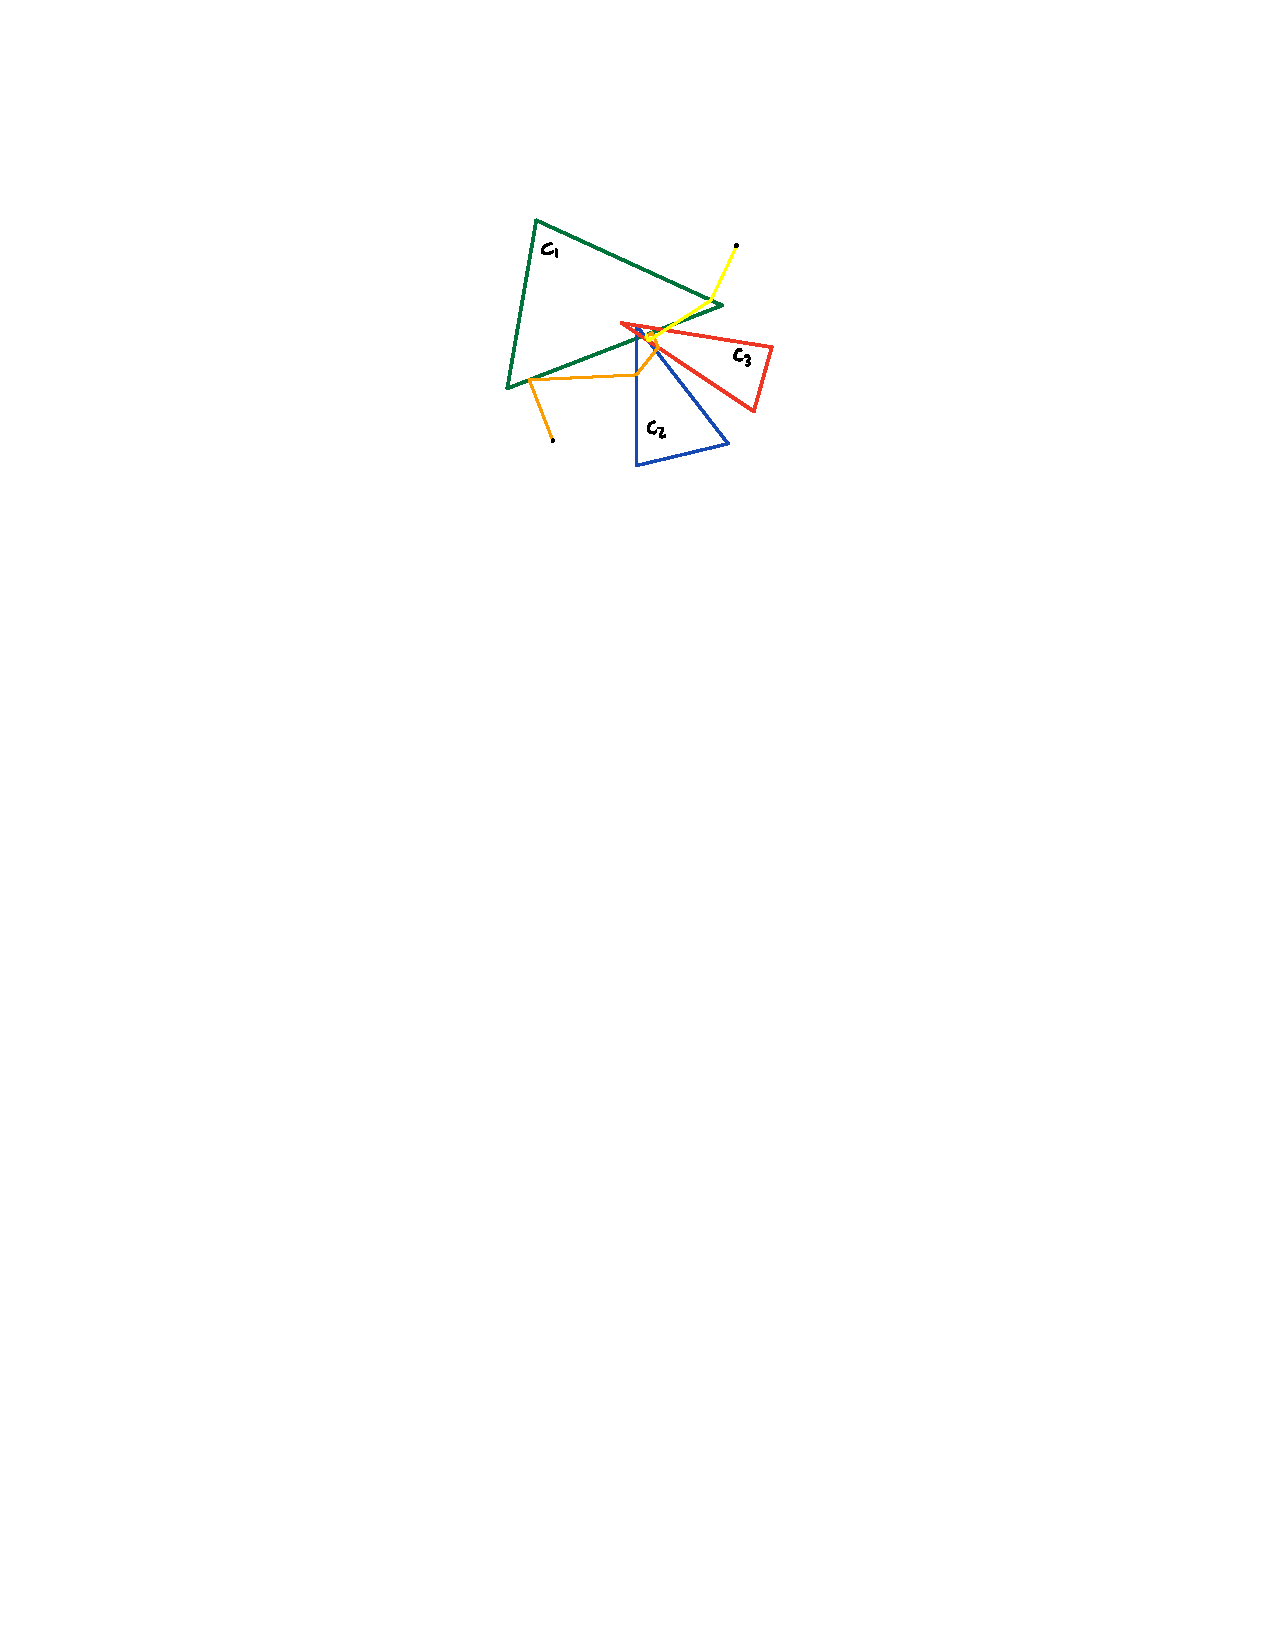
\includegraphics[width=1.25in]{figures/ch4_pocs}
%\vspace{0.5in}

\end{frame}

\begin{frame}{4.6: Orthogonal Projection onto Half Spaces}

\vspace{2mm}

For $\vecnot{w} \in V$, let $H = \{ \vecnot{v} \in V \,|\, \tinner{\vecnot v}{\vecnot w}\geq c \}$ be a closed convex \textcolor{blue}{half space}.

\begin{itemize}
\item For $\vecnot v\in H$, the projection satisfies $P_{H}(\vecnot v)=\vecnot v$ 
\item For $\vecnot v\notin H$, the projection satisfies $P_{H}(\vecnot v)=P_{U+\vecnot v_{0}}(\vecnot v)$ because \\ the closest point in $H$ achieves the inequality with equality
\end{itemize}

\vspace{2mm}

It follows that \vspace{-2.5mm}
\begin{equation*}
P_{H}(\vecnot v)=\begin{cases}
\vecnot v & \text{if }\tinner{\vecnot v}{\vecnot w}\geq c\\
\vecnot v-\frac{\inner{ \vecnot v}{\vecnot w} -c}{\left\Vert \vecnot w\right\Vert ^{2}}\vecnot w & \text{if }\tinner{\vecnot v}{\vecnot w}<c
\end{cases}\label{eq:proj_ineq}
\end{equation*}

\vspace{1mm}
\hrule
\vspace{4mm}
Thus, alternating projection can find a feasible vector $\vecnot{x}\in \mathbb{R}^3$ satisfying \vspace{-1mm}
{\small
\begin{align*}
2x_{1}-x_{2}+x_{3} & \geq-1\\
x_{1}+2x_{3} & \geq2\\
-7x_{1}+4x_{2}-6x_{3} & \geq1\\
-3x_{1}+x_{2}-2x_{3} & \geq0
\end{align*}
}
\vspace{-3mm}

\vspace{-1.1in}
\hspace*{3.7in}
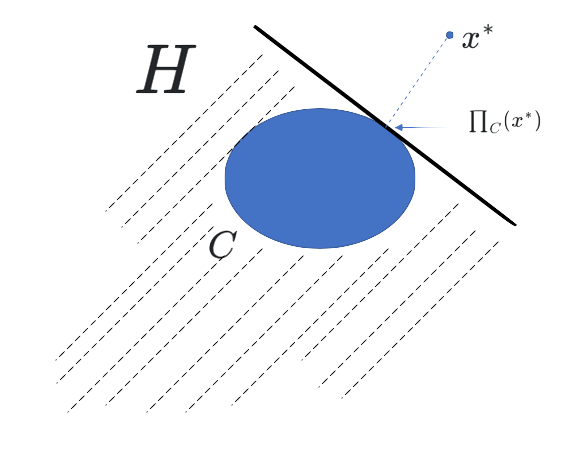
\includegraphics[width=2.2in]{figures/ch4_halfspace}
%\vspace{0.5in}

\end{frame}

\begin{frame} \frametitle{Next Steps}

\begin{itemize}
\setlength\itemsep{5mm}
\item To continue studying after this video -- \vspace{2mm}

\begin{itemize}
 \setlength\itemsep{3mm}
 
 \item Try the required reading:  Course Notes EF 4.6
 
 \item Look at the Mini-Project Handout on Alternating Projection

 \item Also, look at the related problems in Assignments 8 and 9
\end{itemize}
\end{itemize}

\note{
	\vspace{8mm}
	\begin{enumerate}
		\setlength\itemsep{3mm}
		\color{red}
		\item Here are some options to continue learning this material. (read) \\ [2mm]  That's it for today.  So, I'll see you next time.
	\end{enumerate}
}

\end{frame}

\end{document}


